\chapter{Practical Architectures \& Paradigms for Concurrency \& Parallelism in Highly Concurrent Network-Bound Applications}
\lstset{frame=tb,
  language=Python,
  aboveskip=1mm,
  belowskip=1mm,
  showstringspaces=false,
  columns=flexible,
  basicstyle={\small\ttfamily},
  numbers=none,
  numberstyle=\tiny\color{gray},
  keywordstyle=\color{blue},
  commentstyle=\color{dkgreen},
  stringstyle=\color{mauve},
  breaklines=true,
  breakatwhitespace=true,
  tabsize=3
}
This chapter examines architectures and paradigms for concurrency \& parallelism in highly concurrent network-bound applications in great detail. \newline
When developing highly concurrent network-bound applications, the major debate is about the shared-nothing versus the shared-something architectural paradigms. Decisions made in regards to the applied paradigm usually have the highest impact on the scalability and key characteristics of an application. So the first section discusses the essence of the shared-nothing and the shared-something approach as well as their implications on highly concurrent network-bound applications. One subsection introduces the shared-nothing “thread-per-core” model that has emerged in the past years to deal with modern high core count CPUs. Its aim is to deliver efficient multi-core scaling on these CPUs in particular.\newline
Furthermore, the chapter addresses work distribution and scheduling strategies in the implementations of established and upcoming highly concurrent network applications and library abstractions, such as Redis version 6 with I/O threading, KeyDB, NGINX, libuv, Tokio and Glommio. The chapter tries to classify the techniques that these implementations make use of based on queueing models and work distribution algorithms. The consecutive section is devoted to Rust Futures and zero-cost async-await and picks up where the preceding subsections about Tokio and Glommio left off. Futures and async-await enable so-called “green threading” - a paradigm that is common in “higher level” concurrent programming. Rust futures make this paradigm viable for highly concurrent “low level” implementations and are essential for the Rust Libraries Tokio and Glommio. \newline
While the sections, which were already described, are mainly about incorporating thread-level parallelism into highly concurrent network-bound applications, the last section in this chapter “changes perspective” and discusses how such applications can benefit from SIMD. 

\section{Shared-Nothing vs. Shared-Something}
\subsection{Essence}
Whether to use the shared-nothing or the shared-everything architecture or something in-between, deemed “shared-something” in this thesis, is a fundamental question when it comes to developing any highly concurrent server application. \newline
Historically, shared-nothing architecture meant that a “high transaction rate multiprocessor system” does not share memory and disk I/O resources, while a shared-everything system shares both memory and disk I/O resources. Something in-between could be that processors only share either memory access or disk access \cite{stonebraker:shared_nothing} (shared-something). However, nowadays this concept is further abstracted to any kind of logical or physical resource that can be shared between nodes \cite{wikipedia:shared_nothing}. A node can store a finite amount of state and offers a finite amount of computational resources, with both hard limiting the amount of data a node can keep and the throughput it is able to process in practice.
\subsection{Discussion}
Although implementation details differ vastly depending on what flavour of shared-nothing, shared-something or shared-everything is actually meant, some general observations about the disadvantages of the approaches can be made: 
Shared-nothing architectures aim to have no contention on resources simply by not sharing them at all. Therefore, in theory, the throughput of an application using shared-nothing can increase linearly in parallel execution as discussed later in the section about the thread-per-core architecture. In shared-something architectures some resources are  shared by definition, resulting in potential contention on these resources. This might force parts of the application to synchronize, which reduces the part of execution time that can actually benefit from parallel execution. Using Admahl’s law, one can calculate the theoretical upper performance limit depending on the proportion of execution time that benefits from parallel execution and the amount of available executing nodes \cite[13-14]{herlihy:art_of_mp} e.g. CPU cores. Usually, a shared-nothing architecture requires almost no or very little synchronization between nodes, and therefore the theoretical upper performance limit is higher compared to the shared-something architecture. Shared-something architectures usually “pay a penalty” in Amdahl’s law for requiring some sort of synchronization. \newline
However, the efficiency of shared-nothing approaches stands and falls with the “delightfulness” of the problem that the implementation is supposed to solve. In this context “delightful” means that the state can be partitioned into non-overlapping collections so that all transactions on that state are locally sufficient \cite{stonebraker:shared_nothing}, i.e. they can be executed on a single node without the involvement of another node. Depending on the nature of the aforementioned state and the application, partitioning state into non-overlapping collections so that transactions are locally sufficient can become a non-trivial problem to solve. One reason for this is that the amount of stored state should be roughly equal among all nodes. A shared-nothing architecture where, for example, 99\% of the state is kept on a single node defeats the purpose and the benefits of shared-nothing. The same principle also applies to the computational resources of the node. A shared-nothing architecture where 99\% of the computation is performed on a single node would make no sense either. The computational resources should be utilized about equally across all nodes. Shared-nothing databases, such as Redis Cluster, usually use “hash partitioning” \cite[205]{kleppmann:data} to fulfill the goal of evenly distributing the keys and the state among the nodes. However, this does not prevent a highly skewed load distribution \cite{amazon:dynamo}: \newline
If the load is not well-balanced, the nodes whose utilization exceeds that of the other nodes  could become hotspot nodes. 
This is why the shared-nothing architecture might be more prone to hotspot problems depending on data access patterns. The following paragraph provides an example of this:  \newline
Given are a shared-everything database running on a single node and a shared-nothing database running on three equivalent nodes A, B and C. The shared-everything database and the shared-nothing database can achieve a maximum throughput of 250k requests and 300k requests per second respectively. In the shared-nothing database a single node can handle 100k requests per second. The data in the shared-nothing database is partitioned in hash slots. One key, which is located in node A of the shared-nothing database, becomes hot. This key is requested 120k times per second. Consequently, node A is running at its hard limit and is forced to drop requests. Within the same time frame another key becomes hot and is requested 100k times per second. Coincidentally, this key is located in node A, too. Node A can not keep up with serving 100k additional requests per second, because its hard limit is already reached, so it is forced to drop even more requests. While node A is failing to serve all of its requests, node B and C of the shared-nothing database might just be serving 5k requests per second each and thus are underutilized. Although it has a lower absolute maximum throughput than the shared-nothing database, the shared-everything database could in theory serve all the requests perfectly fine in this example.
This is an extreme case and a thought experiment, but skewed workloads are not unusual. For example, when a celebrity on a social media site causes a “storm of activity”, millions of followers might want to access the celebrity's profile, which could internally be represented by an ID that is the key to the profile content in the database. In conclusion, one partition has to deal with the whole workload. Skewed workloads have to be tackled at application level for most databases \cite[205]{kleppmann:data}, e.g. by making the data set more finely grained. \newline
Getting back to the example with the shared-nothing database, it would be the best hypothetical case if the keys and the access to the keys were uniformly distributed among the nodes. \newline
The hotspot problem mentioned above was named as one of the reasons why “Alibaba Cloud” decided to implement a multithreaded fork of Redis despite the possibility of data partitioning via Redis Cluster \cite{alibaba:redis}. \newline
This problem is closely related to queueing theory. Shared-something architectures normally make use of the single-queue, multi-server model, whereas shared-nothing architectures usually make frequent use of a multi-queue, multi-server model. \newline
“Non-delightful” transactions on shared-nothing systems are either not possible at all or they require a transaction protocol and message passing between the nodes. Generally, depending on the latencies between involved nodes and the frequency and execution cost of “non-delightful” transactions, the performance ranges from acceptable to too slow for a viable system.\footnote{Interestingly in shared-something systems the complexity is in the field of concurrency \& parallelism, while in shared-nothing systems the complexity shifts to problems related to distributed computing.}  \newline
The metastate, which contains the information on which node a specific piece of state is stored, also has to be stored somewhere and has to be distributed. \newline
As shared-nothing architectures usually involve more logical nodes than shared-everything architectures, they can introduce more administrative overhead to distributed systems.
In conclusion, if the data and the access patterns meet the requirements for the shared-nothing architecture, its advantages outweigh the benefits of shared-something approaches and it should be preferred. The benefits of the shared-nothing architecture are not limited to “truly” distributed environments. Applications running on modern servers with multi-core CPUs can also benefit from the shared-nothing architecture, which will be demonstrated in the section “Thread-Per-Core” and in the performance evaluations for this study.

\subsection{“Work around” non-delightful Transactions - A Case Study Of Transactions in Redis Cluster}
The in-memory database Redis enables transactions via Lua scripts. Clients can send Lua scripts, which can then be evaluated on the Redis server with specified parameters. Lua scripts are executed transactionally and provide strict serializable isolation guarantees on one Redis server instance \cite{redislabs:rollback}. Redis transactions do not make use of any client interaction within the script, which makes them particularly efficient.
Redis Cluster consists of multiple Redis server instances arranged in a shared-nothing database cluster, where keys are evenly distributed among nodes via hash slots. Redis Cluster does not support distributed transactions. That means transactions in Redis Cluster can never cross the boundary of a single node and thus only involve keys which are all stored on the same Redis server instance. However, to make transactions in Redis Cluster possible, the client can force the involved keys into a single hash slot on a single node by utilizing a concept that Redis calls “hash tags” \cite{redis:cluster}. These “hash tags” ensure that only a substring of the key is hashed for the hash slot by putting it into braces. So, for example, if the keys “foo” and “bar” are involved in a transaction, the substring “baz” can be appended in braces. Only “baz” is hashed for the hash slot and this ensures that “foo\{baz\}” and “bar\{baz\}” end up on the same node, making the transaction possible. The downside of this approach is that it may contribute to worsening the hotspot problem that was described in the previous section.

\subsection{Thread-Per-Core and Amdahl’s law}
To fully utilize the core count of modern multicore CPUs in I/O heavy applications, the thread-per-core architecture was developed. The goal of this architectural approach is to embrace the fact that CPU core speeds do not increase as much anymore, whereas core counts on CPUs increase monotonically. So its focus is on utilizing all available CPU resources. The principle is simple: Create exactly one thread in the application for each available CPU core. The idea is that assigning exactly one thread per core reduces the amount of expensive context switches in the system. \newline
The thread-per-core model works especially well with the shared-nothing architecture because in theory it can scale linearly with the CPU core count in the system:  \newline
\centerline{$S_{latency}(s) = \frac{1}{(1 - p) + \frac{p}{s}}$}
\centerline{Given $p = 1$}
\centerline{$S_{latency}(s) = s$} 
If needed, shared-nothing thread-per-core can make use of “pipe()-style” message passing for inter-thread communication. The time spent on passing messages between processes (or threads) reduces the variable \textit{p}. Communication between processes should thus be used sparsely.  \newline
Shared-something architectures often need synchronization on the shared resources.
Depending on whether this synchronization reduces the proportion p of the time, which profits from parallelization, and depending on how much it is reduced, the theoretical speedup of the program is limited. Therefore, the application does not scale indefinitely on an infinite amount of CPU cores. In reality, this means that with each added CPU core the CPU cores are utilized less efficiently and at some core-count this is not a viable scaling strategy anymore. \newline
The paper “The Impact of Thread-Per-Core” compares a shared-nothing thread-per-core in-memory database with the common multithreaded in-memory database “memcached” running on the same hardware and utilizing the same amount of threads. The paper shows that a shared-nothing thread-per-core approach with configured interrupt request (IRQ) affinity can reduce tail latencies by up to 71\% for in-memory databases  \cite{peassa:thread_per_core}.
When IRQ affinity is enabled, only specific cores in the kernel are responsible for packet processing and receiving interrupts from the NIC. \newline
For inter-thread communication the database described in the paper makes use of a bounded and lock-free circular SPSC queue.

\section{Work Distribution and Scheduling in Highly Concurrent Network-Bound Applications}
Highly concurrent network-bound applications are supposed to take advantage of multicore CPUs, so they need methods for distributing the workload to multiple operating system processes/threads and consequently to the CPU cores. This implies the need for concepts and algorithms for distributing and scheduling the workload.\newline
The workload in highly concurrent network-bound applications is primarily characterized by small tasks, which are issued by a large amount of mostly independent connections and require rather “little” computation and long waiting times in-between I/O operations in most cases. A task in such a system is usually a unit of work which can be executed concurrently. The goal is to achieve high performance by multitasking between tasks efficiently. This section discusses how to achieve parallelism in highly concurrency network-bound applications and points out the strengths and weaknesses of different work distribution and scheduling strategies.\newline
The most trivial scheduling strategy for a network application is to use blocking I/O and assign an OS-thread to each established connection as described earlier. This strategy already enables parallelism. With this approach, it is up to the operating system to unblock and schedule the probably mostly blocked threads and thereby serve the concurrent connections. However, the problem with this approach is that concurrency is enabled via thread-level-parallelism. Processes/threads should not be used to enable plain concurrency, which does not necessarily require parallelism, for multiple reasons: Repeatedly creating operating system processes/threads and lots of context switching, which is required whenever data arrives on one socket, are too expensive for highly concurrent network-bound applications. On modern hardware, one context switch requires about 1-2 microseconds \cite{bendersky:context}. On a 2 GHz CPU core, 2 microseconds equal 1000 CPU cycles. This might not sound like a lot, but in theory, one 2 GHz CPU core has only about 1600 CPU cycles overall to process 1 kilobyte of payload, if the CPU core wants to make full use of the capabilities of a 10 Gbps NIC. 1000 CPU cycles just for a context switch is quite demanding in comparison. \newline
So one thread should handle more than just one connection. The best performance is typically achieved by keeping operating system processes/threads busy with computation that is ensured to make progress and mapping each thread to a CPU core. I/O selectors provided by the operating system and user space network stacks, such as the ones discussed at length in chapter 2, give the application the ability to serve several connections concurrently in an efficient manner, while being agnostic about parallelism within the application in the first place. So the question of how to schedule the tasks driven by the I/O selector and the related processing for several cores efficiently\footnote{Efficiency is not well-defined in this context. It depends on the requirements for the application.} remains.\newline
This section is based on information which can be extracted from the source code and documentations of several open source multithreaded/multi-processed highly concurrent network-bound applications and library abstractions, namingly “NGINX”, “Redis” and “KeyDB”, “libuv”, “Tokio” and “Glommio”. \newline
NGINX is the “Swiss Army knife” of high performance HTTP based applications and a very popular web server, caching server, reverse proxy and load balancer \cite{soft:nginx}, which can often be found at the top of corresponding benchmarking results. KeyDB is a multithreaded fork of the popular in-memory database Redis \cite{soft:keydb}. libuv is a library that provides asynchronous evented I/O, which was originally developed to drive Node.js’ event loop \cite{soft:libuv}. Tokio is a runtime that is focused on asynchronous operations. It serves as a basis for the popular actor framework ACTIX \cite{soft:actix} and Deno \cite{soft:deno}, that is Ryan Dahl’s\footnote{Ryan Dahl developed Node.js in 2009.} new implementation of a Node.js like JavaScript runtime for server applications. Glommio is a thread-per-core I/O library based on the new Linux asynchronous I/O API “io\_uring” \cite{soft:glommio}, which is still in its early stages. \newline
Nowadays, most highly concurrent network-bound applications achieve parallelism by integrating processes/threads into the Reactor Pattern in some way or other. The Reactor Pattern was already mentioned in the second chapter in the first section about I/O notification selectors, but its key concepts will briefly be reviewed as a reminder: \newline In the Reactor Pattern, a handle is an entity of interest, for example a socket. Notifications of specific events on the descriptor, for example read-readiness, can be registered with an I/O notification selector, such as “epoll”, which is usually provided by the operating system. This I/O selector blocks until an event of interest occurs on at least one of the registered handles (file descriptors). A handle has an associated callback function (Event Handler) for each event that can occur on the entity. An Initiation Dispatcher dispatches the callbacks associated with each handler and then goes back to calling the I/O selector (Synchronous Event Demultiplexer) \cite{schmidt:reactor}. This is called an event loop and one iteration within the loop is an event loop tick. This approach is efficient because the thread which runs the event loop either processes events and thus makes progress or it is blocked if there are no events to process. In some documentations, this is also referred to as “event-driven architecture”. The main program logic is completely single-threaded and driven by the event loop in such an architecture. In theory this architecture is rather simple. However, in practice there are usually a few obstacles that one needs to know about for further context: \newline
While the reactor architecture works well for networking operations, file operations on UNIX-like operating systems are technically always “ready” and setting them to non-blocking mode makes no difference as explained earlier. They can potentially always block the thread. So running them on the same thread as the event loop is risky and can potentially reduce the performance severely because the event loop could be prevented from processing events and making progress. The solution is to utilize separate operating system processes/threads for handling file I/O requests. This means that even an application with just a single event loop instance running on one thread requires operating system threads for file I/O. NGINX, KeyDB, libuv and Tokio all make use of this approach for dealing with file I/O. \newline
Often it is desired that UNIX signals can be received via the I/O notifications. While this is possible via the “signalfd” system call \cite{man:signalfd} on Linux nowadays, this behavior can also be achieved by using the “self-pipe trick” \cite[1370-1372]{kerrisk:linuxapi}. \newline
Waking the event loop thread using another process/thread or communicating custom events can be achieved by utilizing the UNIX “pipe” system call. To do so, a pipe has to be created. The read end has to be registered with the I/O selector and the write end can be used in another process/thread for sending arbitrary data. 

\subsection{Producer-Consumer - Redis I/O threading}
Redis' approach to multithreading differs vastly from the approaches of the other mentioned applications and libraries. Redis used to be driven by a completely single-threaded reactor until Redis version 6. By default Redis is still single-threaded, but since version 6 it is possible to manually enable I/O threading. The idea is that the event loop still runs on only one thread, but instead of handling all synchronous reads and writes to the clients’ sockets on the thread that runs the event loop, reads and writes are queued and postponed to be processed by multiple I/O threads. The schematic in figure \ref{fig:redisio_arch} shows a visual representation of Redis’ I/O threading.\newline
In simplified terms, the main thread, which runs the event loop, is the only producer in the system and the I/O threads implement multiple consumers for fan-out socket I/O operations. The main thread waits synchronously for the consumer threads to finish.
\begin{figure}
  \centering
  \scalebox{0.7}{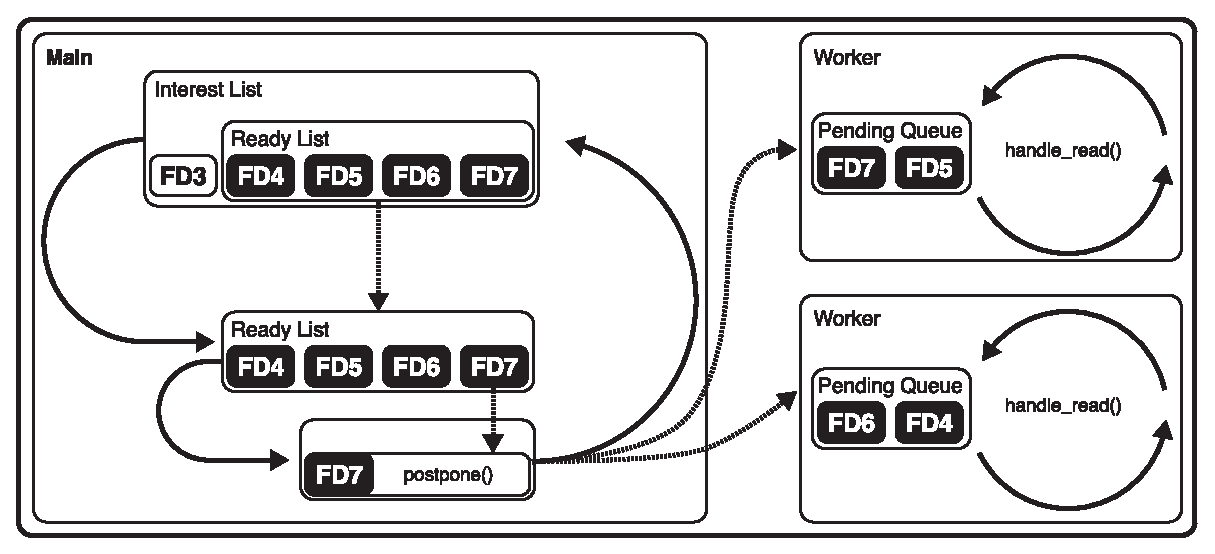
\includegraphics{./figs/redis/redisio_arch}}
  \caption{Simplified schematic of producer-consumer I/O threading in Redis.}
  \label{fig:redisio_arch}
\end{figure}
The reasoning behind this design choice is that under full load Redis spends the majority of the computation time on I/O operations specifically reading from and writing to sockets \cite{antirez:io_threading}. By benchmarking GET and SET operations, I could verify that with payloads up to the smaller kilobyte range Redis spends about 80\% of computation time on reading from and writing to TCP sockets under full load. Redis I/O threading is supposed to benefit from parallelizing this part by utilizing a producer-consumer model, which distributes the read and write tasks across consumer threads. The number of I/O consumer threads is specified in the configuration file or with an option flag at startup. \newline
However, there is a caveat regarding the implementation: The I/O consumer threads are not always active. Instead, they are “woken up” by unlocking a corresponding mutex for each consumer on the main thread when a certain load threshold is reached. If the I/O threads are active and the workload is below the threshold, the consumer threads are blocked by locking the corresponding mutexes on the main thread. When they are awake, the threads are busy-looping and waiting for work by checking if the length of their work queue is non-zero. The main thread distributes clients with pending read or write tasks evenly among these separate queues on each event loop tick. When the work is distributed, the main thread sets the length of each of the consumer queues atomically. This signals the consumers to stop spinning and start processing I/O. After that, the main thread processes its own slice of clients. When the main thread is finished, it synchronously waits until all consumers have finished their work. To find out if all consumers have finished their work, the main thread “busy-checks” if the total sum of the queues’ length is zero. The pseudocode for Redis’ I/O threading is displayed in figure \ref{fig:redisio_code}. The threads are busy-waiting because waking them up by unlocking the mutex on each event loop tick would be too expensive. Spinning threads do not have to be woken up but they have the disadvantage of "burning" CPU cycles, especially if there is no or little work to do. So the I/O threading is only activated when there is enough work to process. It is advisable to never set the number of I/O threads higher than the number of available CPU cores. The operating system does not “know” if a thread is just busy-looping or actually making progress. It could interrupt the thread running the event loop to schedule an equal time slice to a thread that is just spinning and waiting for work from the main event loop thread, which could potentially degrade performance. This could also happen if there are more available CPU cores than I/O threads. However, this is unlikely if there is no other significant load on the system. To rule this problem out completely, it is also possible to pin the threads to specific cores. For the reasons mentioned above, Linus Torvalds advises against the usage of spinlocks in user space altogether \cite{torvalds:spinlock}.
\begin{figure}
  \centering
  \begin{lstlisting}
while !shutdown:
    handle_pending_reads_using_threads(global_read_queue)
    handle_pending_writes_using_threads(global_write_queue)
    # using stateful event notification interface e.g. epoll
    events = stateful_poll_wait(stateful_poll_fd, timeout)
    for event in events:
        if event.fd == listener_fd:
            event.fd.accept()
        if event.mask & READABLE:
            # will postpone read if I/O threads active
            connections[event.fd].handle_read_event()
        if event.mask & WRITABLE:
            # interest is registered (rarely) if write was previously blocking
            # due to level-triggered notifications
            connections[event.fd].handle_write_event()

# producer side (main thread)
handle_pending_writes_using_threads(global_write_queue):
    i = 0
    # distribute work
    for write_task in global_write_queue:
        thread_queues[i++ % thread_count].push_back(write_task)
    # "fan-out" - give the go to the worker I/O threads
    for thread_id = 0; thread < thread_count; thread_id++:
        thread_pending[thread_id].atomic_store(thread_queues[thread_id].length)
    # meanwhile main thread (id = 0) handles its slice
    while write_task = thread_queues[0].pop():
        handle_pending_write(write_task)
        thread_pending[0]--
    # "join" - busy-waiting for the other threads to finish their work
    while sum(thread_pending) != 0
\end{lstlisting}
\pagebreak
\begin{lstlisting}
# consumer side (spinning worker threads)
thread_create(
    # note: in the real implementation this thread can be blocked
    # by a mutex that is controlled by the main thread
    while True:
        # busy-waiting for write task from the queue
        while thread_pending[thread_id].atomic_load() == 0
        # thread handles its slice
        while write_task = thread_queues[thread_id].pop():
            handle_pending_write(write_task)
            thread_pending[thread_id]--
, thread_count - 1)
\end{lstlisting}
  \caption{Simplified pseudocode for producer-consumer I/O threading in Redis.}
  \label{fig:redisio_code}
\end{figure}
\pagebreak
\subsection{Multithreaded Event Loop(s) - NGINX, KeyDB, libuv and co.}
\begin{figure}
  \centering
  \scalebox{0.7}{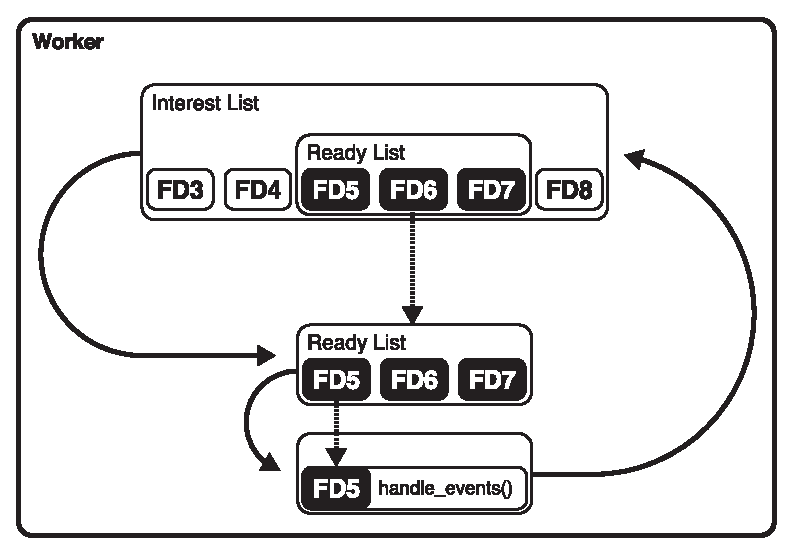
\includegraphics{./figs/keydb/keydb_arch}}
  \caption{Simplified schematic of one worker in KeyDB's multithreaded event loop(s).}
  \label{fig:keydb_arch}
\end{figure}
The general concept for scaling to multiple cores in NGINX, KeyDB, libuv and Tokio is running the reactor logic with the event loop on multiple operating system threads/processes.  \newline
There are, however, subtle differences in the technical implementations regarding the usage of “epoll” and other I/O notification systems. The scheduling of the work also differs and for some of the implementations this is not the only paradigm for achieving parallel processing besides file I/O. \newline
To put it simply, the NIC can be seen as the producer and the threads running the event loop as the consumers. The interface between them is a (stateful) I/O selector provided by the operating system. In the case of “epoll”, the “epoll” instance created with “epoll\_create” can be seen as the work queue. By calling “epoll\_wait” the threads running the event loop pop  multiple tasks off of that work queue. The first distinction between the implementations is that this “main” work queue, which distributes the work on each event loop tick, can either be shared or non-shared. KeyDB and NGINX have a work queue and therefore an “epoll” instance per worker thread/process on Linux, while Tokio shares the “epoll” instance.\footnote{Redis, which forms the basis for KeyDB fork, does not use edge-triggered but level-triggered notifications and so does KeyDB. Level-triggered notifications are complicated to use with one shared “epoll” instance. As mentioned previously, edge-triggered notifications are preferred in this use case. This might also have influenced the decision to implement one “epoll” instance per worker thread in KeyDB.} The schematic in figure \ref{fig:keydb_arch} shows a visual representation of a single worker thread in KeyDB’s multithreaded event loop. The corresponding pseudocode is displayed in figure \ref{fig:keydb_code}.  \newline
Conceptually, both approaches have advantages and disadvantages. The reason why both approaches are in use boils down to queueing theory: A single queue, which is shared across workers, leads to a better distribution of the work and consequently to potentially lower latencies and higher throughput. In theory, the single-queue, multi-server is deemed superior over the multi-queue, multi-server system \cite{prasad:server}. In a single-queue, multiple-server scenario, a comparably demanding task does not actively prevent successive work in the queue from being processed. The “blocking” effect is also known as “head-of-line blocking” \cite[17-18]{kleppmann:data}. \newline
In the case of “epoll” with edge-triggered notifications, things are not that simple though. Calling “epoll\_wait” pops multiple events with associated tasks off of the “work queue”. A reactor style application then processes a whole batch of tasks associated with the events synchronously. So one demanding task within that batch can still “head-of-line-block” successive tasks from being processed, but subsequent tasks, which are added after popping the tasks off of the ready queue\footnote{So basically which are added \textbf{after} calling “epoll\_wait”.}, are not directly affected by the processing time required for a demanding task in the batch. In most server applications not all workloads, which are generated by those batches, are equal, but in some use cases a high load in comparison to the "batch size" may make this problem insignificant. \newline
Leveraging a shared work queue across multiple threads still tackles the problem of evenly distributing work during runtime to some degree and is therefore already a form of dynamic work assignment. Threads which have completed their work call the stateful I/O selector to pick up a new batch of work from the shared queue, which supports threads that are still busy and processing events. \newline
On the other hand, the principle “one queue per worker thread” eliminates the contention on the queues and generally renders the need for sharing any state of connections with other threads obsolete because each worker only receives the notifications for its own subset of connections. As each worker serves its own subset of connections, there is the need for a concept for assigning these connections to the threads. The assignment of the connections is static in the case of KeyDB, so the algorithm is rather simple: Saturate the threshold of C connections on each of the N worker threads. When the threshold is saturated on all workers, each connection is “round-robin” distributed, so that it is assigned to one of the worker threads with the fewest connections. This threshold can and should probably be optimized for the use case in production.\footnote{For my benchmarks I set this threshold to one.} Once a connection is assigned to a specific worker, it cannot move to another worker. So this kind of work distribution is not influenced by the actual load on the workers. This creates a similar problem as discussed in the section about shared-nothing architectures: \newline
If the work is almost uniform randomly distributed among the connections, this static work assignment is probably ideal because it creates no overhead during runtime after the connection was assigned to the worker thread. However, if that is not the case, work might be distributed unevenly, which could lead to worse throughput and latencies, especially in high load scenarios. \newline
NGINX has the ability to start multiple worker processes and analogous to KeyDB, each worker process has a reactor with its own stateful system selector instance (e.g. epoll instance). Connections are distributed by the kernel in NGINX. The listener socket is duplicated on “fork()” and therefore shared among the processes. In scenarios with smaller load in Linux this leads to the kernel handing most new connections to the same worker process because Linux unblocks the last thread that called “epoll\_wait”. This worker process accepts and serves the requests, resulting in comparably high load on that one worker process. To achieve fair scheduling, it is possible to use the “SO\_REUSEPORT” option on Linux \cite{man:socket}. “SO\_REUSEPORT” makes it possible to create a new socket that listens on a port which is already in use. Thus a new socket structure in the kernel is created. The kernel “round-robin” queues incoming connections onto socket structures. So when each worker has its own socket structure, connections are distributed “round-robin” as a consequence. However, this can produce a higher variance on response times compared to the conventional “dup” on the same socket structure \cite{majkowski:nginx}. Sharing the listener socket structure corresponds to a single-queue, multi-server model, while creating a socket structure for each worker corresponds to a multi-queue, multi-server model. So the results are in line with the theoretical superiority of the single-queue, multi-server model.  \newline
Creating multiple event loops in “libuv” also results in multiple “epoll” instances and therefore multiple work queues similar to KeyDB’s and NGINX’s approach. However, the library libuv also offers another paradigm for introducing parallelism to the Reactor Pattern: 
As mentioned previously, all of these programs/libraries use threads for dealing with file I/O. These threads are usually implemented as thread pools. Thread pools have the advantage of setting an upper limit for running threads and threads within the pool do not need to be created and destroyed repeatedly, which is an expensive operation in the context of high performance server applications \cite[370-371]{herlihy:art_of_mp}. Depending on the threads’ stack size, these advantages usually come at a relatively low memory usage trade-off. 
“libuv” makes it possible for the application to queue arbitrary work onto these thread pools, using the “uv\_queue\_work” function. “uv\_queue\_work” takes a data pointer for sharing state, a work callback, which can contain “blocking” computation, and a completion callback. In this context “blocking” refers to computations that make the event loop wait long enough, and thus “blocks” the event loop from processing events and making progress, which is the reason why it should be offloaded. This could be “real” thread blocking computations, such as an external library, which makes use of blocking file descriptors, but also something computation-intensive like request sanitizing, for example.
\begin{figure}
  \centering
  \begin{lstlisting}
thread_create(
        while !shutdown:
            # process pending writes from queue
            # on EAGAIN install write handler
            handle_pending_writes(event_loops[thread_id].write_queue)
            # using stateful event notification interface e.g. epoll
            # each worker thread runs its own event loop with a dedicated stateful_poll instance
            events = stateful_poll_wait(event_loops[thread_id].stateful_poll_fd, timeout)
            # synchronous event demultiplexing
            for event in events:
                if event.fd == event_loops[thread_id].listener_fd:
                    # distributes connections to matching thread
                    event.fd.accept_on_thread()
                if event.mask & READABLE:
                    # when query is executed push result into the pending write queue
                    event_loops[thread_id].connections[event.fd].handle_read_event()
                if event.mask & WRITABLE:
                    # interest is registered (rarely) if write was
                    # previously blocking due to level-triggered notifications
                    event_loops[thread_id].connections[event.fd].handle_write_event()
, thread_count)
\end{lstlisting}
  \caption{Simplified pseudocode for KeyDB's multithreaded event loop(s).}
  \label{fig:keydb_code}
\end{figure}

\subsection{Work Stealing Scheduling - Tokio}
In comparison to KeyDB, NGINX and libuv, the asynchronous runtime Tokio has a more sophisticated architecture:\footnote{Tokio’s runtime has a modular design and offers different runtime strategies. Depending on the use case, it can be built with the different feature sets. This thesis generally refers only to the multithreaded Tokio runtime with enabled network functionality, which is Tokio’s default.  \newline
It should also be noted that Tokio is still a relatively young project and the API was only recently stabilized with the 1.0 version in December 2020. From my experience, a lot of information on implementation details one can find on the internet is outdated and should be taken with a grain of salt. The code in the mainline is the only source that can be trusted. Tokio is probably the most complex and ambitious project of all the projects addressed in this thesis, so it can be quite hard to grasp the essential logic that drives Tokio by taking a quick glance at the source code.}  \newline
Tokio is written entirely in Rust and differs from the other approaches that were mentioned in the way that it embraces concurrent programming by leveraging the concept of lightweight Rust futures. Other “higher level” asynchronous runtimes, such as the runtime of the popular Go programming language, often use fibers\footnote{Also known as stackful coroutines} instead. “Futures” deserve their own section, but to put it simply, they act as a proxy for computation that has yet to happen. In Tokio a task logically represents a chain of non-blocking futures that is scheduled cooperatively in user space by “yielding” back to the runtime. Tasks are a unit of work that can be run concurrently. The Go equivalent of a Tokio Task would be the “goroutine”. This concept is also known as “green threading” or N:M threading. Similarly to “goroutines", Tokio Tasks can communicate via channels \cite{doc:tokio_task}. Tokio is included in this section because the futures within its tasks are state machines generated at compile time, which are dynamically scheduled at runtime by a relatively lightweight scheduler, bringing the performance of applications developed with Tokio to a level comparable to what “system-level” implementations, such as the previously mentioned applications and library abstractions in this section, offer. This section focuses on the reactor and scheduling in Tokio. The reactor uses one instance of a stateful I/O selector such as “epoll” with edge-triggered notifications and shares it among the worker threads. So Tokio leverages the single-queue, multi-server approach, which is superior to the multi-queue, multi-server approach in theory, in regards to “epoll”. However, the difference is that the thread, which receives the batch of ready events by calling the I/O notification selector, does not necessarily dispatch the associated callbacks directly. Instead the thread calls the “wake” method of the ready descriptors. The call to “wake” pushes the associated task into the run queue of the worker which provided the “waker”. Each worker thread has its own bounded run queue for runnable tasks. When this queue is full, work is pushed onto a global multiple-producer, multiple-consumer queue. By default, the Tokio runtime spawns one of these worker threads per CPU core, so Tokio also embraces the thread-per-core model. Each worker pops off tasks of its own run queue and processes them by polling the top-level future of each task until the queue is empty. When the queue is empty, the worker tries to “steal” half the tasks of every other worker onto its own run queue, starting with a random worker. If the worker succeeds in “stealing” half the tasks of at least one of the other workers, the worker continues the processing of tasks. If it does not succeed, it falls back to checking the global queue for tasks. In either case, after the worker successfully “stole” tasks, it goes back to processing the new tasks in its own run queue before calling the I/O notification selector. In case no worker has any tasks that could be stolen, the worker calls into this selector for new I/O notifications immediately and starts the next event loop tick. As a side effect, tasks are generally processed within one global event loop tick. Figure \ref{fig:tokio_arch} shows a simplified schematic of Tokio’s main components and the different worker states.
\begin{figure}
  \centering
  \scalebox{0.7}{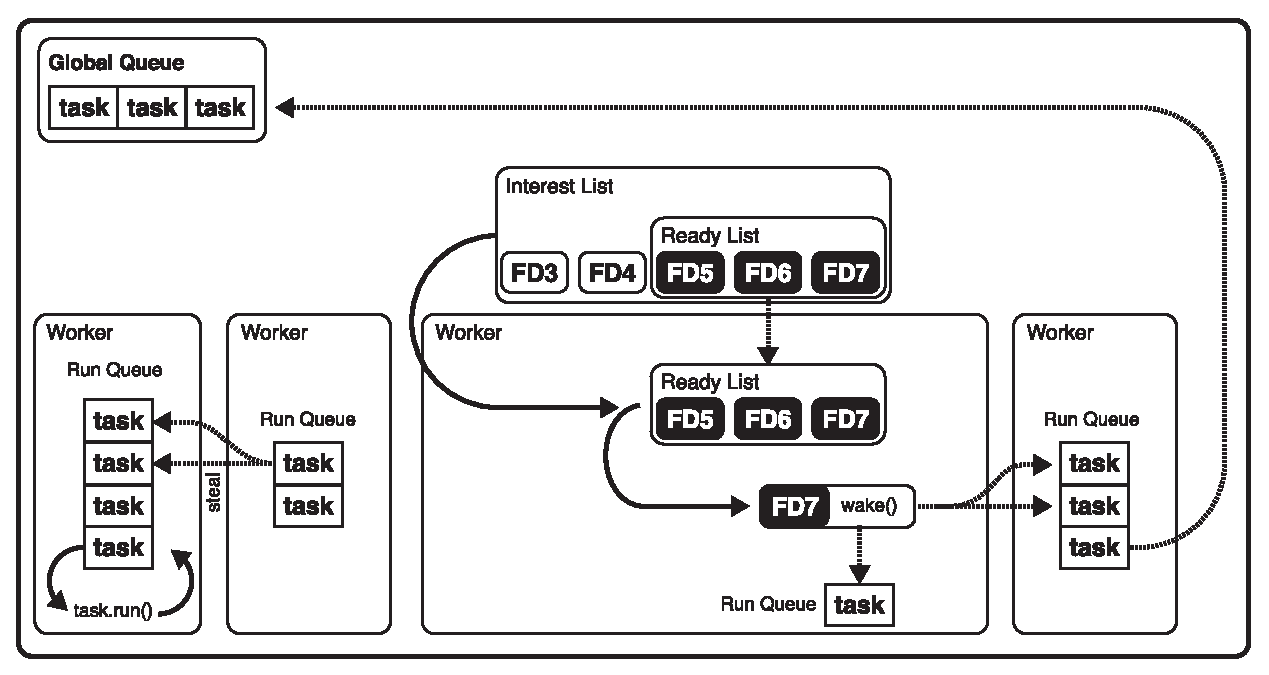
\includegraphics{./figs/tokio/tokio_arch}}
  \caption{Simplified schematic of Tokio's main components and the different worker states.}
  \label{fig:tokio_arch}
\end{figure}
By implementing this work stealing dynamic scheduler, Tokio tackles one of the problems described earlier:  \newline
The I/O notification selector returns a “batch of work” under load, so even though the shared “epoll” instance with edge-triggered notifications is essentially a shared queue, workers  receive multiple tasks from that queue at once. A scheduled task, which requires relatively long computation, can still block tasks scheduled for later execution within the run queue of a worker thread (head-of-line blocking). One solution to this problem could be to push \textbf{all} the tasks onto a single shared queue and let N consumer worker threads pop off one task at the time. However, the Tokio developers ruled this solution out due to relatively high contention on a single queue \cite{lerche:scheduler}. That is the reason why in the Tokio implementation each worker has its own local run queue to work around the contention on a global queue. To counteract the disadvantages of a local queue, underutilized workers with an empty work queue “steal” from workers which still have runnable tasks. This “work stealing scheduling” counters underutilization, potentially decreases queueing delays the “stolen” tasks might face otherwise, and generally contributes to more uniform load distribution among worker threads. The goal of work stealing is to optimize for busy workers that make progress without generating too much overhead in the common case \cite[380]{herlihy:art_of_mp}. So making the process of workers popping tasks off of their own local queue as cheap as possible is key to avoid bottlenecks that are caused by the scheduling. However, it is acceptable if “stealing” from another worker’s queue is a more demanding operation in comparison. The queue implemented by Tokio is a bounded circular SPMC queue, which is very similar to the SPSC queue presented in the section about concurrent queues and memory barriers. The main difference is that because this SPMC queue implementation allows for concurrent dequeuing, it requires an atomic CAS operation in the pop method to make sure that the updated head is only “released” and the task is returned, if no other thread has concurrently updated the head. \newline
One more issue Tokio tackles is the granularity of the tasks: A uniform and comparatively fine granularity of tasks reduces the complexity of fair scheduling and makes the runtime more predictable. So the team behind Tokio suggests that developers insert yield points, which give control back to the scheduler, in between relatively demanding computations in their applications and libraries if possible \cite{ryhl:async}.\newline 
Alternatively, computationally intensive or blocking computations can be offloaded to a thread outside of Tokio’s thread pool with the “spawn\_blocking” function. The result of the blocking computation can be non-blocking asynchronously awaited until completion within a Tokio task that runs on a normal worker thread.\footnote{The effect is similar to the “uv\_queue\_work” function in libuv.} \newline
In Tokio each “await” within a future on another asynchronous future is also a potential yield point. The worker drives the chain of futures of each task in the run queue until it cannot continue making progress. As a result in certain conditions the worker may continuously poll a task’s futures for a comparably long time until one future in the chain is not ready anymore. \newline
For example, if there is a large socket buffer in the kernel that is ready to be read from and the read buffer in user space is relatively small in comparison, a loop within the future of the task, which reads from the socket, does not break and yield to the worker’s scheduler until the socket buffer is drained (EAGAIN). To reduce the effect of such a “not-yielding” task, which can lead to “head-of-line blocking”, the Tokio runtime assigns an operation budget to each task per “event loop tick”. This operation budget is a simple integer, which is decremented with each poll on a task’s future. When this counter is zero, the task automatically yields to the worker’s scheduler. The Tokio authors claim that adding this operation budget reduced response time percentiles to a third of their original values in some cases \cite{lerche:preemption}.\newline The pseudocode in figure \ref{fig:tokio_code} demonstrates the main logic that drives the Tokio runtime.\newline
\begin{figure}
  \centering
  \begin{lstlisting}
thread_create(
        while !shutdown:
            # poll on each (probably) ready future
            # for progress until the run queue is empty
            while task = run_queue.pop():
                task.future.poll(&context)
                # as long as there is budget remaining and
                # a task exists in the "lifo_slot" keep polling.
                budget = INITIAL_BUDGET
                while lifo_task = lifo_slot.take():
                    if !budget--:
                        run_queue.push_back(lifo_task)
                        break
                    lifo_task.future.poll(&context)
            # try stealing work from the other workers
            if try_steal_into(&run_queue):
                # if successful continue
                continue
            # check for work in the global queue
            if task_global = global_queue.pop():
                # if successful continue
                run_queue.push_back(task_global)
                continue
            # using stateful event notification interface e.g. epoll
            # reactor with shared stateful_poll instance
            # on event on fd wake the corresponding tasks
            events = stateful_poll_wait(stateful_poll_fd, timeout)
            for event in events:
                # wake will push each associated task into the
                # run queue of the responsible worker
                global_scheduled_io_ressources[event].wake()
, thread_count)
\end{lstlisting}
  \caption{Simplified pseudocode for Tokio's work stealing scheduler.}
  \label{fig:tokio_code}
\end{figure}
The Tokio runtime is supposed to be a compromise between fair scheduling, whose goal is to distribute load uniformly among all the available cores, and high throughput performance.
Multiple benchmarks of ACTIX-web, which makes use of Tokio, against other HTTP frameworks can be found on the internet and it seems to perform very well \cite{andre:tokio}. Some benchmarks even claim that ACTIX’s throughput is two times higher than that of equivalent Go implementations and that its performance in response times is also better \cite{techempower:tokio}. \newline
In a uniform load scenario the maximum throughput of Tokio is probably slightly lower compared to approaches where work distribution is rather static, like in KeyDB, due to the user space scheduling overhead. However, when the load produced by connections is non-uniform, Tokio should in theory yield improved tail latency results, which can mainly be attributed to the work stealing scheduling strategy and the limited task operation budget per tick. In some cases overall throughput might increase as well due to a better utilization of the available CPU cores.  \newline
Tokio’s developers have implemented an incomplete Redis server (and client) named Mini-Redis \cite{soft:miniredis}. This application is rather a “toy”, which serves to demonstrate some of the capabilities and features of Tokio. As it comes in handy, the benchmarks in chapter 4 include Mini-Redis, but the results should be taken with a grain of salt because deep optimizations are certainly not the highest priority in a “showcase application”.  

\subsection{Thread-Per-Core and io\_uring - Glommio}
Glommio is a young thread-per-core I/O library, which is written in Rust just like Tokio and also ships with a runtime focused on asynchronous computation and based on lightweight Rust futures. It should be noted that Glommio is currently in its early stages of development. It is the only library mentioned in this chapter that already takes advantage of the new asynchronous I/O API “io\_uring”, which is available only for Linux at the moment\footnote{January 2021}. Unlike Tokio, Glommio embraces the shared-nothing architecture. So similar to KeyDB each worker runs a completely independent event loop. In Glommio, the way this event loop works vastly differs from how it works in the previously mentioned implementations because of the truly asynchronous programming paradigm of the “io\_uring” API. The reactor registers three “io\_uring” instances per CPU core in Glommio: The main ring, which should be used for the main I/O operations, the latency ring for low latency I/O operations and the poll ring, whose main focus is polling fast storage devices, such as NVMe flash memory drives, for data. So Glommio relies on the multi-queue, multi-server model, which, in theory, is the inferior model, but has the advantage of no contention on the queues in practice .  \newline
This is important because the goal of Glommio’s shared-nothing thread-per-core architecture is almost linear scaling and contention would hinder the achievement of this goal. 
\footnote{Modern x86-64 Server CPUs usually have some sort of simultaneous multithreading (SMT), which results in two vCPU cores per CPU core. On a x86-64 CPU with enabled SMT one CPU core would be responsible for six “io\_uring” instances in this architecture. It would also be interesting to see how the kernel handles the large amount of rings in a system with a high CPU core count and the effect of enabled IRQ affinity.}  \newline
Glommio’s runtime is similar to Tokio’s in that both rely on cooperative scheduling. Developers can create task queues with varying “shares”. The “shares” are used to proportionally assign CPU time under load. The more “shares” a queue has, the more CPU time is given to the queue. The function “yield\_if\_needed” should be deployed within large tasks to yield control back to the scheduler. “yield\_if\_needed” checks if there is pending data to process at the latency ring. Since “io\_uring” maps the submission and completion rings into user \textbf{and} kernel space, this operation is a lightweight integer comparison of head and tail values at the “latency completion ring”. No system call is required. Latency sensitive events in this latency ring can be prioritized over events in the main ring. When there are no events on either of the rings, Glommio registers notifications for the latency ring’s file descriptor with the main ring and the thread can safely be blocked by calling “io\_uring\_enter”. It is up to the developer to properly configure the tasks with regard to computation time and latency requirements. The previously mentioned applications and library abstractions do not actively prioritize certain tasks over others, but rather try to complete all tasks with the lowest latency possible. This is a paradigm shift in Glommio. Finding the right latency requirements for a use case in a potentially large distributed fan-out architecture in the first place and mapping these use cases to the proper underlying tasks in Glommio is a non-trivial problem. In the case of Glommio the concept of encapsulation is partially abandoned in exchange for a better performance.  \newline
In shared-nothing architectures like Glommio, state is usually partioned. Consequently, in a database application, which is split by key ranges, the state where each key range is stored\footnote{In real implementations this is probably rather a hash slot than a key range.} also has to be kept somewhere. In Redis Cluster this state is stored on the clients and each node has its own independent listener port because it is a “standalone” Redis server instance. Consequently each Redis’ Cluster client establishes a connection with each node in the cluster. In the shared-nothing thread-per-core database, which is mentioned in the section about the thread-per-core paradigm, the state is stored on the database server and queries are redirected to the responsible thread via user space message passing. The advantage of this approach is that the server can listen on a single port, thus clients establish only a single connection to the database. \newline
A database developed with Glommio could also listen on a single port by creating a separate non-shared listener socket for each thread using the “SO\_REUSEPORT” in Linux \cite{man:socket}. “SO\_REUSEPORT” makes it possible for each listener socket to have its own queue, although the listener sockets “listen” on the same port. As discussed in the section about NGINX, incoming connections are distributed “round-robin” onto the queues of these dedicated socket structures. However, the Glommio database would not use message passing to redirect queries. Instead, Glommio’s developer suggests to make use of “extended Berkeley Packet Filter” (eBPF) programs in the kernel to process and route each packet to the corresponding socket structure and thread, which is responsible for the key \cite{glommio:ebpf}. In essence eBPF programs can “hook” into designated code paths in the kernel and execute custom logic. The eBPF code itself runs safely inside of a virtual machine  \cite{lwn:ebpf}. So the process of routing to the corresponding socket is handled entirely within the kernel. Therefore no redirection in user space is required.

\section{Rust Futures and zero-cost async-await}
Highly concurrent network-bound applications try to fully capitalize on the provided hardware. However, “lower level” languages such as C and C++, which are closer to the hardware, do not ship with any abstractions or ecosystems that support the implementation of high concurrency applications. Furthermore, they are usually considered rather “unsafe” to work with for reasons that are beyond the scope of this study. So entire language ecosystems have been built on the premise of simplifying concurrent programming, such as Erlang or Golang. They all give up some control over the hardware for improved ergonomics and safety, such as a garbage collected runtime\footnote{Garbage collection can be particularly problematic, because it can have a negative impact on tail latency results.} and higher level concepts like “fibers” for green-threading, which usually create overhead. The Rust ecosystem provides a proof of concept that highly concurrent and highly performant close-to-hardware code does not have to be “ugly” or “unsafe”. In fact, one of Rust’s core features besides a performance similar to C/C++ and “memory-safety at compile-time” is “fearless concurrency”. In Rust one of the fundamental building blocks of concurrency, which is especially relevant for network applications, is the concept of futures and zero-cost async-await.  \newline
Futures are data structures that act as a proxy for the result of a computation that is not yet complete \cite{wikipedia:futures}. Rust’s “future ecosystem” is implemented as zero-cost abstractions and should be considered when building high performance applications, such as highly concurrent network-bound server applications. In practice, the “Future trait”\footnote{“Interfaces“ in other imperative programming languages are similar to Rust’s “traits”.}  provides the possibility to implement efficient concurrency that “asynchronous runtimes”, such as Tokio or Glommio, can rely on.  \newline
When Rust futures are polled they either resolve the result of the computation or return “pending”, which signals that the computation is not ready yet. Consequently, each future has to implement a poll method, which is the function that drives the future’s progress and that either returns the enum type “Poll::Ready” containing the result\footnote{“Enums” in Rust can store entire structures, so these “enums” can serve as union types, too.} or “Poll::Pending” \cite{man:std_future}.  \newline
Rust’s futures are the foundation for Rust’s async-await syntax. Rust’s async-await syntax is syntactic sugar for composing one “big” future out of multiple futures. Each “await” represents a poll on a future in the chain and a possible yield point.  \newline
“Async” functions are transformed at compile time into functions which return a future. The returned future is essentially a generator, which is created at compile time and then turned into an optimal state machine. This state machine contains all the necessary data within the states and the logic for acting upon that state for driving the futures. Conceptually, the state machine is a union type over all possible states and therefore its memory footprint is roughly the size of the largest state. Mapping variables within an “async” function to the states efficiently requires a liveness analysis. \newline
The basic concept behind the liveness analysis is that for each variable at each yield point it ensures within an “async” function, that the variable is stored within one or multiple states, if it can prove that a value written to the variable before the yield point\footnote{Each yield point is a possible state transition.} might be read after the state transition. If two variables within an “async” function are in use at the same time, the memory that stores the two variables within the states must be non-overlapping \cite{mandry:await}. \newline
However, the async-await syntax hides all of that complexity from the programmer and by chaining futures makes composing asynchronous logic trivial, while not sacrificing the performance of the application by leveraging zero-cost abstractions and compile time optimizations. \newline
Futures in Rust are “lazy” and cannot make progress without being polled. This strategy is optimal for enabling concurrency on a single processor \cite{bahe:garbage_collection}.
The executor, which itself might be driven by a reactor like in Tokio, is responsible for polling the top-level future owned by a task at the right time by calling the poll method and passing a “context”. However, nothing happens if a future is polled when the computation is not ready yet, apart from wasting CPU time. A needless poll just returns “pending”. The context that is passed as an argument to the poll function of the future contains a “waker”. This waker is responsible for notifying the executor once the corresponding task is ready to be polled and is passed with each poll because futures can be moved to different tasks with a different waker. When the executor is notified it has to poll the top level future of the task at least once to ensure that it can continue to make progress \cite{rust:asyncbook}.\newline
Network applications usually deal with streams of data. Streams in Rust’s future ecosystem represent a series of values that are produced asynchronously, so they are essentially futures that can yield multiple asynchronous results \cite{man:crate_future}. One use case for a stream could be a TCP connection.

\section{SIMD for Network Applications}
Multiprocessing is not the only way to achieve parallelism on modern CPUs. As the name suggests SIMD (single instruction, multiple data) allows the computer to execute the same operation on multiple data points in parallel. Modern instruction set architectures (ISAs), such as x86-64 and ARMv8, offer a set of SIMD instructions and corresponding registers for applying the same operation to a vector of packed integer or floating point values with a single instruction. This approach is more efficient than executing the same instruction multiple times sequentially and therefore leads to better performance and higher energy efficiency \cite{kagan:mmx, henpat:computer_arch}. \newline
SIMD instructions were added to Intel x86 CPUs in the form of the MultiMedia eXtension (MMX) in 1997. These instructions were originally targeted, at high demanding multimedia applications, such as 3D applications and videos, to speed up the vector math. In the following decades Intel added several iterations of Streaming SIMD Extensions (SSE) and later Advanced Vector Extensions (AVX) to their x86 CPUs, with each major iteration adding more and wider registers as well as more instructions \cite{man:avx}. Latest generation Intel CPUs have 32 512-bit wide AVX-512 registers per CPU core.\newline
Modern compiler backends such as LLVM or the GCC backend can do their best to substitute operations on normal arrays with SIMD instructions automatically. In the case of Clang and GCC such “auto-vectorization” optimizations are applied on optimization level three (flag “-O3”) by default or manually with flag “-ftree-vectorize” enabled \cite{doc:llvm_vec, doc:gcc_vec}. \newline
The best way to make sure that certain logic in the application truly benefits from SIMD is to optimize the code in assembly “by hand” or alternatively use “SIMD intrinsics”. This might also require rearranging the data structure layout. The best case for SIMD computation is the structure of arrays (SoA) processing method as the structure’s data can be loaded directly into SIMD registers, while the more traditional array of structures (AoS) arrangement often requires loading data from non-contiguous memory into a SIMD register \cite{intel:soaaos}. Modern vector architectures support non-contiguous loads, so-called gathers, but they come along with a trade-off in performance compared to contiguous loads \cite{henpat:computer_arch}. \newline
Almost all x86-64 CPUs in use today support AVX2 and can therefore load one half of a cache-line into a 256-bit wide register and compare the values of two registers at 32 bytes each with one instruction in parallel, for example. The application of SIMD is not limited to conventional vector math. This provides the opportunity for significantly improving performance on string or buffer operations, such as protocol and query parsing or table scans, which are common in network applications. In the past years, research has been done regarding efficient vectorizing of such algorithms. \newline
The hash table\footnote{Also known as hash map or dictionary} is a standard data container that has a use case in almost every network application. For example, a single Redis server instance instantiates 95 hash tables on startup and the core database is implemented as a hash table. \newline
A few years ago Google noticed that significant portions of the execution time in their applications is spent with processing hash tables. So Google started implementing their own family of more optimized hash tables named “swiss tables". Before that Google mainly used the hash tables from the C++ standard template library such as “std::unorderd\_map”. In typical hashmap implementations linked lists or tree structures are used to chain entries when hash entry collisions occur. This leads to cache misses on typical operations. The “absl::flat\_hash\_map” of the Google “swiss tables”, on the other hand, is implemented as a flat probing table with a seperate array, which contains a byte of metadata for each entry in the table. Each metadata byte contains 7 bits of the 64 bit hash code of the key of the corresponding entry and 1 bit which is reserved to signal if the entry is empty, full or deleted. The other 57 bits of hash code are used to find the start of the “bucket chain” in the probing table. The slice in the metadata array, which contains the metadata of the corresponding entry, fits entirely into the first level cache and is scanned using SSE instructions with 16 candidates in parallel \cite{doc:swisstable}. The find operation on the hash table returns the matching candidate or candidates. Because seven bits of the hash code already match, the requested entry is likely among the candidates. Google claims that the migration to the optimized “swiss hash tables” reduced the percentage of fleet-wide CPU utilization by half a percent, while RAM was reduced by about one percent \cite{kulukundis:swisstable}.
\newline Network applications often spend a considerable amount of time parsing data exchange formats such as the JavaScript Object Notation (JSON). Historically, JSON parsing was mainly done character by character in most implementations. The library “simdjson” changes this paradigm and instead implements a JSON parser that makes use of SIMD and branchless programming techniques to parse whole vectors of bytes on a single core in parallel. On a modern Intel x86 Skylake CPU “simdjson” is able to parse multiple gigabytes of data on one core. This results in a 2.1 times speedup when parsing the “Twitter JSON benchmark” compared to other popular open-source implementations \cite{langdale:simdjson}.
\footnote{Redis and KeyDB do not utilize SIMD for protocol and query parsing at this point in time. There is no information suggesting that NGINX makes use of SIMD for parsing HTTP. Especially in NGINX, SIMD might be a great opportunity for potential performance improvements.} \newline
Bloom filters are probabilistic data structures that can be used to efficiently check if a value is (probably) present in a set of values. They have many possible purposes in network driven applications, such as databases. For example, they are useful to speed up look-ups in sorted string tables (SSTables). Polychroniou’s et al. 2014 paper “Vectorized Bloom Filters for Advanced SIMD Processors” describes the results of tests conducted to find out how the use of SIMD on Bloom filters affects the performance. The tests demonstrated a speed up of “bloom filter probing” by 1.4 to 3.3 times using Intel AVX2 SIMD instructions \cite{polross:bloom}. \newline
Network applications using SIMD can definitely benefit from parallelism on a single core. Generally, when data is processed in a loop and iterations are not directly dependent, vectorization utilizing SIMD might be profitable. However, it should be noted that this often requires a complete change in the way programmers think about algorithms and data structures. Algorithms heavily relying on SIMD are often hard to comprehend at first glance because programmers are usually not used to this model. One good example of this is the “simdjson” project.
